\documentclass{article}
\usepackage{authblk}
\usepackage{hyperref}
\hypersetup{
    colorlinks,
    citecolor=black,
    filecolor=black,
    linkcolor=black,
    urlcolor=black
}
\usepackage{pdfpages}
\includepdfset{pagecommand={\thispagestyle{plain}}}

\begin{document}
\pagestyle{plain}
%%%%%%%%%%%%%%%%%%%%%%%%%%%
% 表紙
%%%%%%%%%%%%%%%%%%%%%%%%%%%
\thispagestyle{empty}
\noindent

\rule{\textwidth}{1pt}
\vspace{2pt}
\begin{flushright}
 \Huge
\begin{tabular}{@{}l}
Core Challenge 2022\\
Solver and Graph Descriptions\\[6pt]
{\Large Version 0.1}
\end{tabular}
\end{flushright}
\vspace{2pt}
\rule{\textwidth}{1pt}
\vspace{10em}


\centering
{\Large Edited by}\\[2em]

{\huge Takehide Soh}\\[0.5em]
{\Large Kobe University, Japan}\\[2em]
{\huge Yoshio Okamoto}\\[0.5em]
{\Large The University of Electro-Communications, Japan}\\[2em]
{\huge Takehiro Ito}\\[0.5em]
{\Large Tohoku University, Japan}\\


%%%%%%%%%%%%%%%%%%%%%%%%%%%
% Table of contents
%%%%%%%%%%%%%%%%%%%%%%%%%%%
\newpage
\tableofcontents

%%%%%%%%%%%%%%%%%%%%%%%%%%%
% Solver Contents
%%%%%%%%%%%%%%%%%%%%%%%%%%%
\newpage
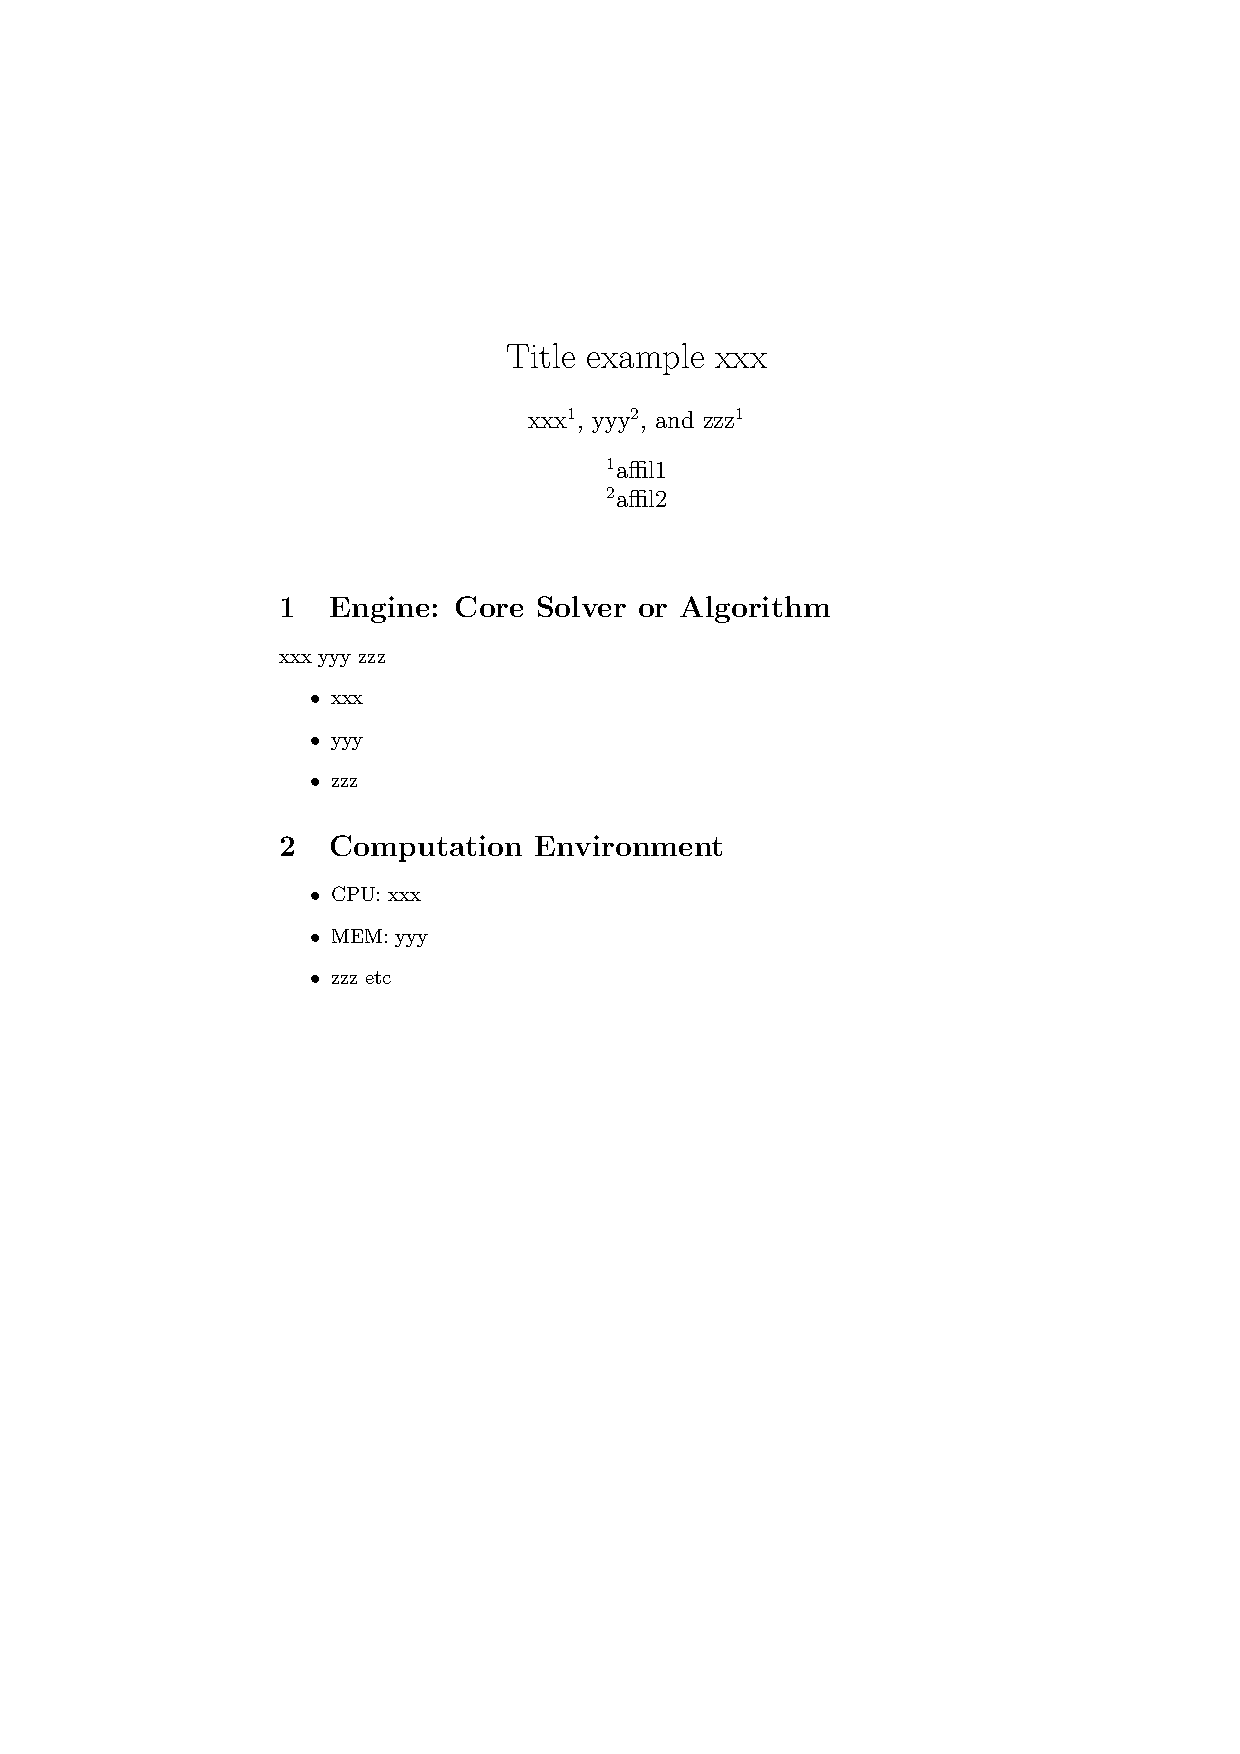
\includepdf[addtotoc={1, section, 1, Title example xxx, lbl:sub1}]{example/example.pdf}


\end{document}
